%%%%%%%%%%%%%%%%%%%%%%%%%%%%%%%%%%%%%%%%%
% Beamer Presentation
% LaTeX Template
% Version 1.0 (10/11/12)
%
% This template has been downloaded from:
% http://www.LaTeXTemplates.com
%
% License:
% CC BY-NC-SA 3.0 (http://creativecommons.org/licenses/by-nc-sa/3.0/)
%
%%%%%%%%%%%%%%%%%%%%%%%%%%%%%%%%%%%%%%%%%

%----------------------------------------------------------------------------------------
%	PACKAGES AND THEMES
%----------------------------------------------------------------------------------------

\documentclass{beamer}

\mode<presentation> {

% The Beamer class comes with a number of default slide themes
% which change the colors and layouts of slides. Below this is a list
% of all the themes, uncomment each in turn to see what they look like.

%\usetheme{default}
%\usetheme{AnnArbor}
%\usetheme{Antibes}
%\usetheme{Bergen}
\usetheme{Berkeley}
%\usetheme{Berlin}
%\usetheme{Boadilla}
%\usetheme{CambridgeUS}
%\usetheme{Copenhagen}
%\usetheme{Darmstadt}
%\usetheme{Dresden}
%\usetheme{Frankfurt}
%\usetheme{Goettingen}
%\usetheme{Hannover}
%\usetheme{Ilmenau}
%\usetheme{JuanLesPins}
%\usetheme{Luebeck}
%\usetheme{Madrid}
%\usetheme{Malmoe}
%\usetheme{Marburg}
%\usetheme{Montpellier}
%\usetheme{PaloAlto}
%\usetheme{Pittsburgh}
%\usetheme{Rochester}
%\usetheme{Singapore}
%\usetheme{Szeged}
%\usetheme{Warsaw}

% As well as themes, the Beamer class has a number of color themes
% for any slide theme. Uncomment each of these in turn to see how it
% changes the colors of your current slide theme.

%\usecolortheme{albatross}
%\usecolortheme{beaver}
%\usecolortheme{beetle}
%\usecolortheme{crane}
%\usecolortheme{dolphin}
%\usecolortheme{dove}
%\usecolortheme{fly}
%\usecolortheme{lily}
%\usecolortheme{orchid}
%\usecolortheme{rose}
%\usecolortheme{seagull}
%\usecolortheme{seahorse}
%\usecolortheme{whale}
%\usecolortheme{wolverine}

%\setbeamertemplate{footline} % To remove the footer line in all slides uncomment this line
%\setbeamertemplate{footline}[page number] % To replace the footer line in all slides with a simple slide count uncomment this line

%\setbeamertemplate{navigation symbols}{} % To remove the navigation symbols from the bottom of all slides uncomment this line
}
\usepackage{setspace}
\usepackage{graphicx} % Allows including images
\usepackage{booktabs} % Allows the use of \toprule, \midrule and \bottomrule in tables
\setbeamertemplate{caption}[numbered]
%----------------------------------------------------------------------------------------
%	TITLE PAGE
%----------------------------------------------------------------------------------------

\title[]{Loop Acceleration For Tightly-Coupled CPU+FPGA System} 
\author[]{
    Cheng Liu 
    \\Supervisor: Dr. Hayden Kwok-Hay So 
    \\Co-supervisor: Dr. Ngai Wong}
\institute {
    Department of Electrical and Electronic Engineering 
    \\The University of Hong Kong
\medskip
}
\date{\today} % Date, can be changed to a custom date

\graphicspath{{./figures/}} 
\begin{document}

\begin{frame}
\titlepage % Print the title page as the first slide
\end{frame}

%----------------------------------------------------------------------------------------
%	PRESENTATION SLIDES
%----------------------------------------------------------------------------------------

%------------------------------------------------
\section{Background} 
%------------------------------------------------
\begin{frame}[t]
\frametitle{FPGA vs. CPU vs. GPU}

\vspace{-1em}
\textbf{FPGA has competitive computation capability and \\
        energy efficiency.} 

\begin{figure}
  \vspace{-1em}
  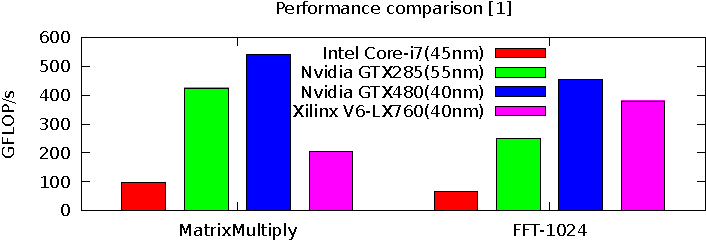
\includegraphics[width=.8\linewidth]{performance-cpu-fpga-gpu}
  \vspace{-1em}
\end{figure}
\begin{figure}
  \vspace{-1em}
  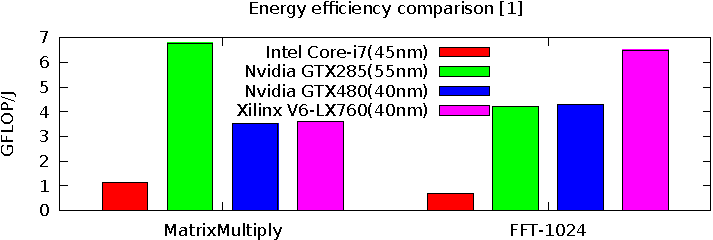
\includegraphics[width=.8\linewidth]{energy-cpu-fpga-gpu}
  \vspace{-1em}
\end{figure}

\begin{spacing}{1.2}
\tiny{[1] Eric S. Chung, etc., Single-Chip Heterogeneous Computing: Does the future include customized
logic, FPGA and GPGPUs?, IEEE International Symposium of Microarchitecture, 2010}
\end{spacing}

\end{frame}

%------------------------------------------------
\section{Related work}
%------------------------------------------------
\begin{frame}[t]
\frametitle{Challenges and progress on FPGA computing}

\vspace{-1em}
\textbf{Challenges}
\begin{itemize}
\item High barrier-to-entry (Hardware knowledge, ...)
\item Low design productivity (Low abstarction level, long compilation time, ...)
\end{itemize}

\textbf{Progress}
\begin{itemize}

\item High level synthesis (HLS), e.g., LegUp, AotoESL, Impulse-C, ROCCC, ...

\item Virtual overlays
\footnotesize
\begin{itemize}
\item[\checkmark] Reconfigurable many-core, e.g., MARC, WPPA(Weakly programmable processor array), ...
\item[\checkmark] Coarse-grained reconfigurable array, e.g.,QUKU, SCGRA, Heterogeneous CGRA, ... 
\item[\checkmark] Virtual FPGA, e.g., Intermediate Fabric, ZUMA, CARBON, MALIBU, ...
\end{itemize}
\normalsize 

\item Other techniques, e.g., Partial reconfigurable technique, Hard Macros, Communication library, ...

\end{itemize}
\end{frame}

%------------------------------------------------
\begin{frame}[t]
\frametitle{Differences and relations of the overlays}

\begin{figure}
\vspace{-1em}
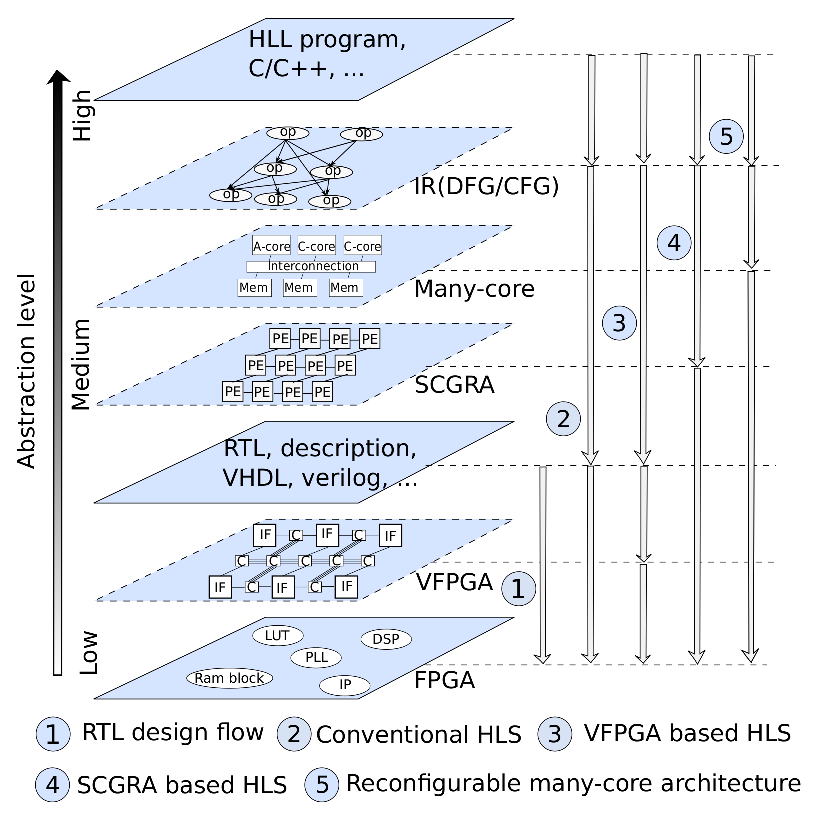
\includegraphics[width=.7\linewidth]{virtual-overlay}
\end{figure}

\end{frame}

%------------------------------------------------
\begin{frame}[t]
\frametitle{SCGRA work in our group}

\vspace{-1em}
\textbf{What have been done?}
\begin{itemize}
\item Introduced the SCGRA layer for HLS,
\item showed potential design productivity improvement,
\item and proved its energy efficiency using an application specific SCGRA topology
\end{itemize}

\textbf{What are still missing?}
\begin{itemize}
\item The relationship between a holistic loop and its kernel data flow graph,
\item influence of the communication between CPU and FPGA on the SCGRA based HLS.
\end{itemize}

\textbf{Focus of my work}
\begin{itemize}
\item Automatic loop acceleration on a tightly-coupled CPU+FPGA using the SCGRA overlay
\end{itemize}
\end{frame}

%------------------------------------------------
\begin{frame}[t]
\frametitle{Why loop acceleration?}

\vspace{-1em}
\textbf{Loop and computation kernel}
\begin{itemize}
\item Loops usually form the most computationally intensive kernel of a program
\item Regularity of loops provide ample of data parallelism
\item Loops are important optimization targets for the parallel computing architecturs including
Multi-core processor, GPU, CGRA and FPGA.
\end{itemize}

\textbf{Difference from previous work}
\begin{itemize}
\item Hardware infrastructure (SCGRA and communication) is changing with the loop optimization
\begin{itemize}
\item[\checkmark] Not possible with hard CGRA
\item[\checkmark] Take advantage of the softness of the FPGA
\item[\checkmark] Application-specific buffering, loop unrolling, and scheduling
\end{itemize}
\end{itemize}

\end{frame}

%------------------------------------------------
\section{Research scheme}
%------------------------------------------------
\begin{frame}[t]
\frametitle{SCGRA based accelerator design flow}

\begin{figure}
\vspace{-1em}
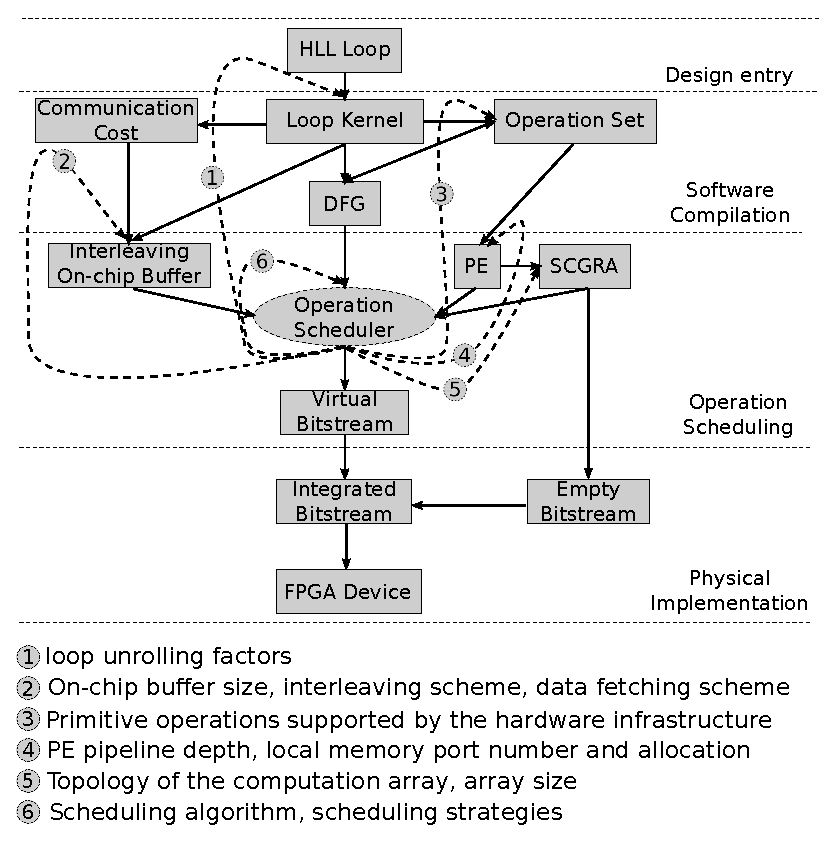
\includegraphics[width=0.76\linewidth]{design-space-overview2}
\end{figure}

\end{frame}

%------------------------------------------------
\begin{frame}[t]
\frametitle{Optimal loop unrolling}

\vspace{-1em}
\textbf{Why loop unrolling and why not fully unroll the loop?}
\begin{itemize}
\item Increases parallel operations and improves performance
\item Induces larger hardware overhead
\item Benefit may be limited by system constrains.
\end{itemize}

\textbf{Loop unrolling problem}
\begin{itemize}
\item Assumptions: Bounded loop, and data dependency known at compiling
\item Input: Sequential program proportition, kernel DFG, loop iteration bound, ...
\item Optimization target: Min(loop execution time/communication cost)
\item Constrain: hardware overhead, IO bandwidth 
\item Model: Operation Scheduling model+Data prefetching model
\end{itemize}
\end{frame}

%------------------------------------------------
\begin{frame}[t]
\frametitle{Hardware infrastructure} 
\textbf{SCGRA based CPU+FPGA accelerator}
\begin{figure}
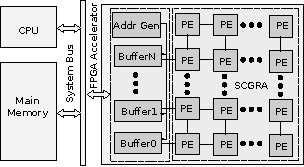
\includegraphics[width=0.65\linewidth]{scgra-acceleratorv2}
\end{figure}

\textbf{Softness of the accelerator}
\begin{itemize}
\item SCGRA structure could be reconfigurable
\item On chip buffer could be reconfigurable
\end{itemize}
\end{frame}

%------------------------------------------------
\begin{frame}[t]
\frametitle{On-chip buffering}

\begin{figure}
\vspace{-1em}
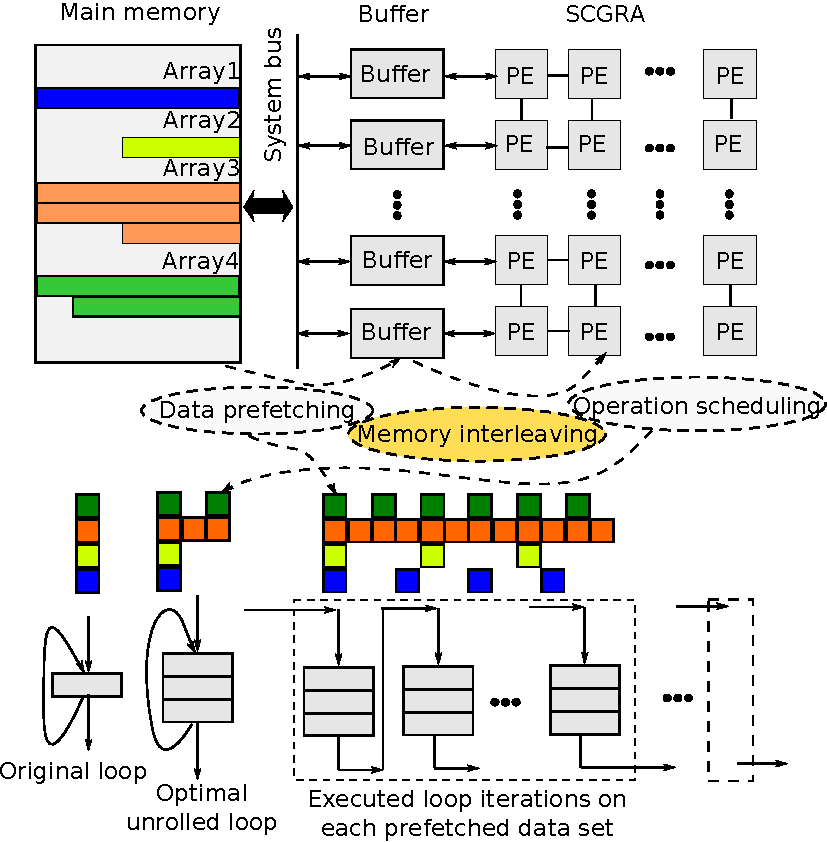
\includegraphics[width=0.7\linewidth]{on-chip-buffer}
\end{figure}

\end{frame}

%------------------------------------------------
\section{Current progress}
\begin{frame}[t]
\frametitle{SCGRA based HLS optimization for both design productivity and frequency}

\vspace{-1em}
\textbf{Optimized SCGRA based HLS}
\begin{figure}
\vspace{-1em}
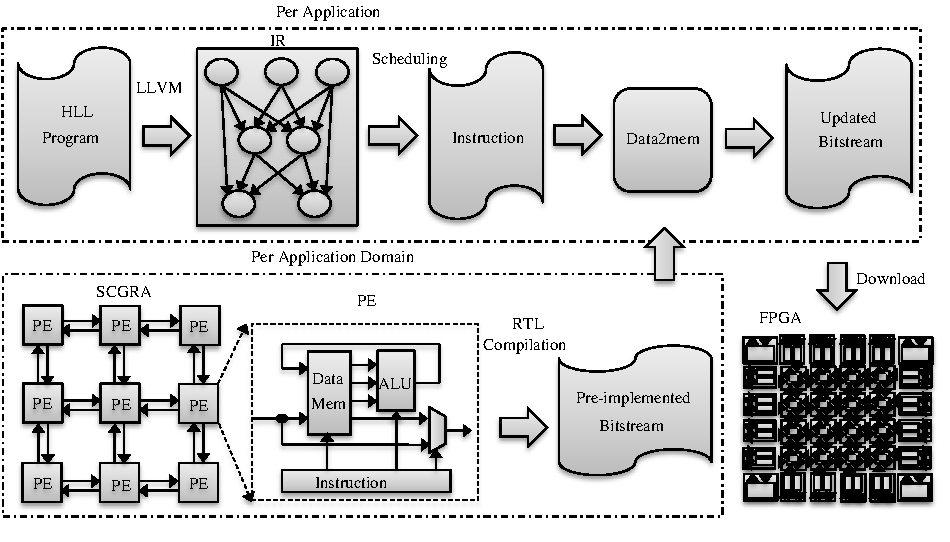
\includegraphics[width=0.75\linewidth]{design-flow}
\vspace{-1em}
\end{figure}

\textbf{Experiment results}
\begin{figure}
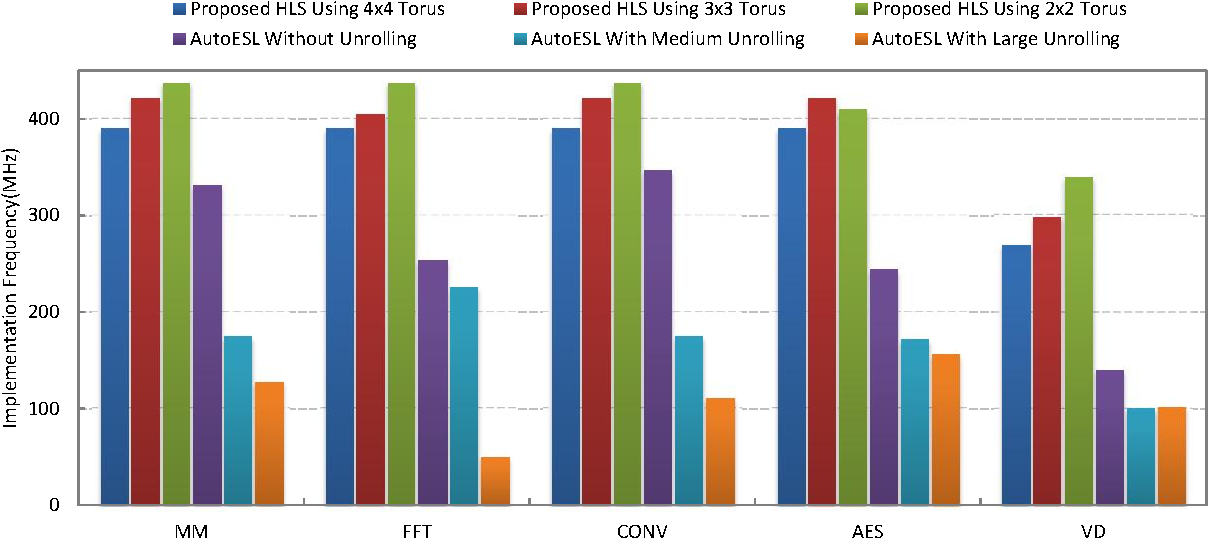
\includegraphics[width=0.5\linewidth]{impl_freq}
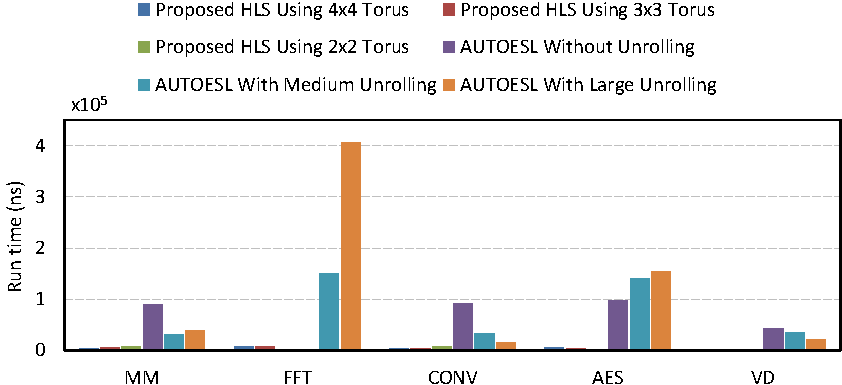
\includegraphics[width=0.5\linewidth]{performanceCP}
\end{figure}

\end{frame}

%------------------------------------------------
\begin{frame}[t]
\frametitle{Preliminary loop unrolling analysis}

\vspace{-1em}
\textbf{loop unrolling influence on performance and overhead}
\begin{figure}
\vspace{-1em}
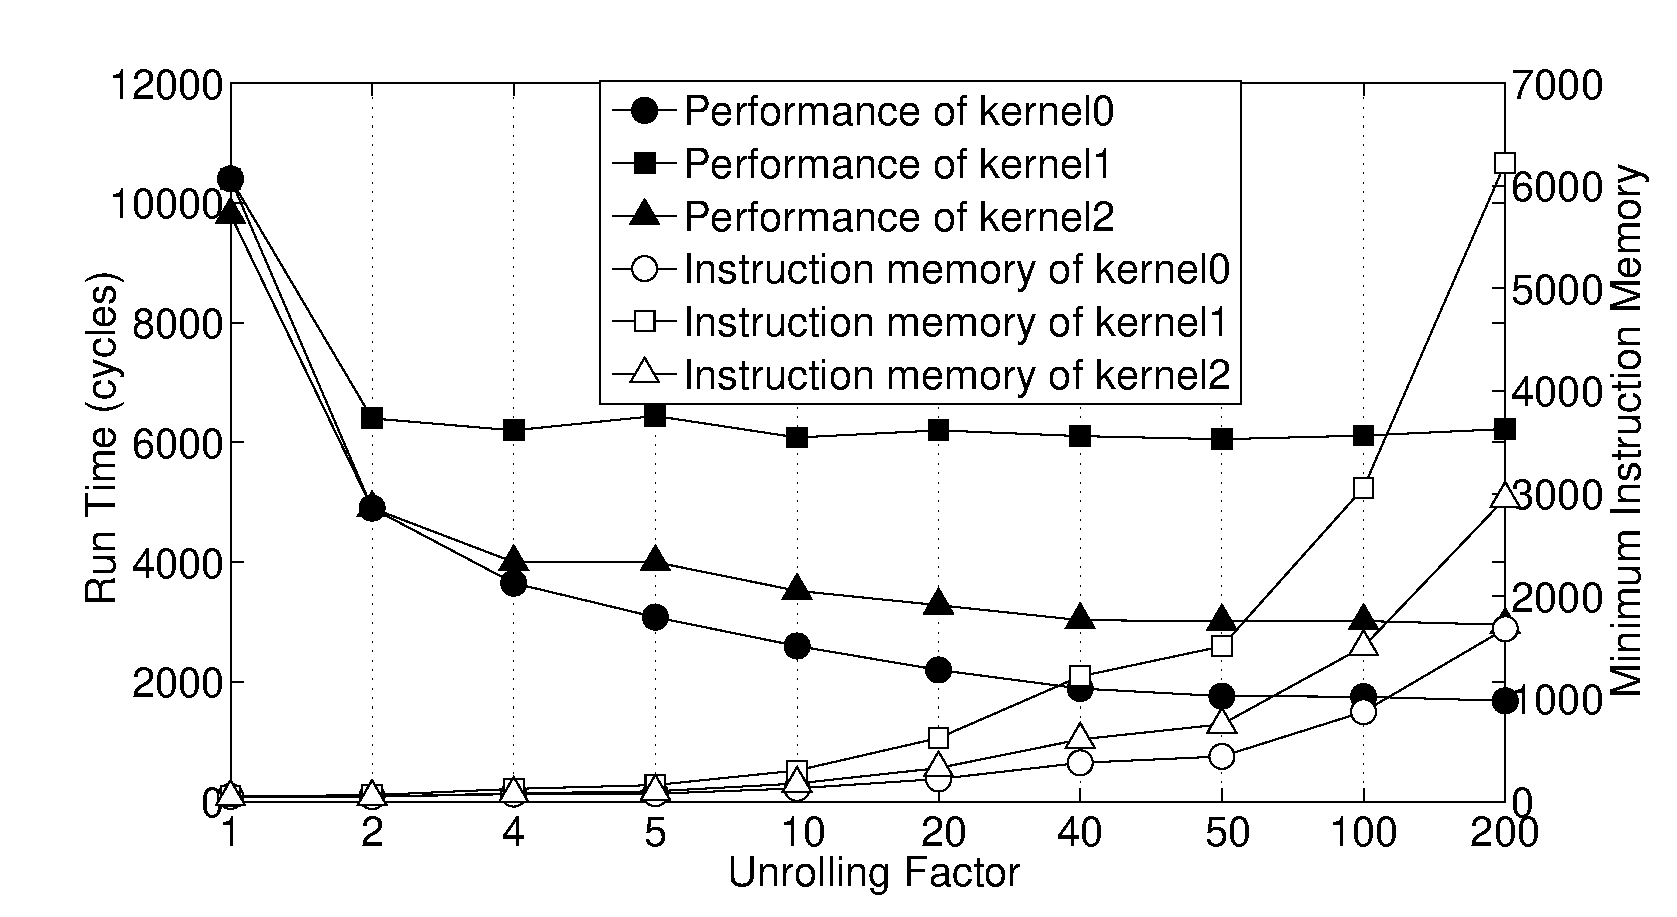
\includegraphics[width=0.6\linewidth]{loop-unrolling}
\vspace{-1em}
\end{figure}

\textbf{Irregular loop bound}
\begin{figure}
\vspace{-1em}
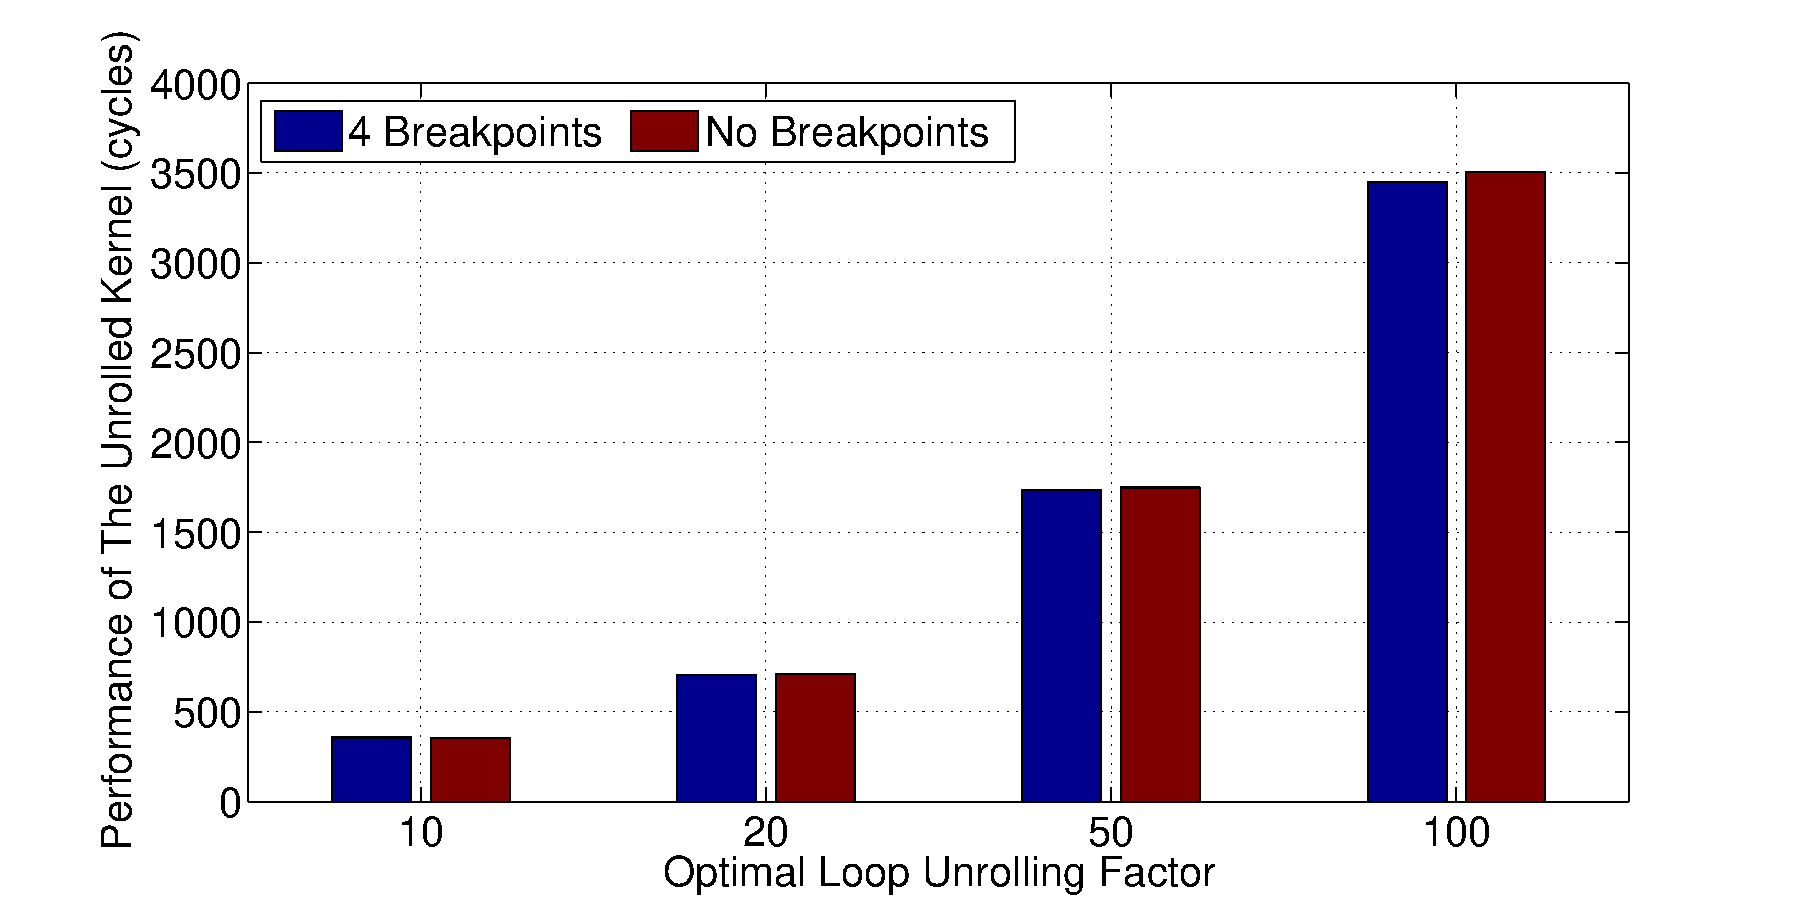
\includegraphics[width=0.6\linewidth]{any-loop-unrolling}
\vspace{-1em}
\end{figure}
\end{frame}

%------------------------------------------------
\begin{frame}[t]
\frametitle{HW/SW communication on Zedboard}

\vspace{-1em}
\textbf{Zedboard platform}
\begin{figure}
\includegraphics[width=0.7\linewidth]{zynq}
\end{figure}
\textbf{Different communication methods}
\begin{itemize}
\item Accelerator coherence port
\item Central DMA, Video DMA, XDMA
\item GPIO
\end{itemize}

\end{frame}

%------------------------------------------------
\section{Conclusion}
\begin{frame}[t]
\frametitle{Conclusion}

\vspace{-1em}
\textbf{Potential contribution}
\begin{itemize}
\item Analyze the relationship between loop and its kernel data flow graph. Hopefully, an optimal
partial loop unrolling may help resolve the BRAM-consuming problem in previous work.  
\item Provide a systemic solution to loop acceleration on a CPU+FPGA system and therefore a more friendly
high level interface to the end users.
\end{itemize}

\end{frame}

%------------------------------------------------

\end{document} 
